\documentclass[11pt,border=5pt]{standalone}
\usepackage{fontspec}
\setmainfont{cmunrm.otf}[BoldFont=cmunbx.otf,ItalicFont=cmunti.otf,BoldItalicFont=cmunbi.otf]
\usepackage{amsmath}
\usepackage{unicode-math}
\setmathfont{NewCMMath-Regular.otf}
\usepackage{tikz}
\usetikzlibrary{arrows.meta,patterns,angles,quotes}
\begin{document}
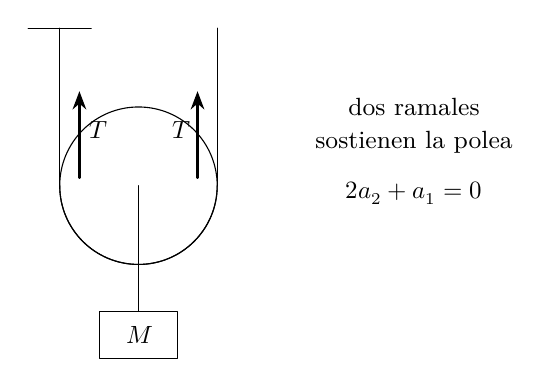
\begin{tikzpicture}[>=Stealth,font=\small,line cap=round,line join=round]
\draw (-1,2)--(-1,0);\draw (-1,0) arc (180:360:1);\draw (1,0)--(1,2);\draw (-1.4,2)--(-.6,2);\draw (0,0) circle (1);
\draw[] (0,0) -- (0,-1.6);
\draw[fill=white] (-0.5,-2.1999999999999997) rectangle (0.5,-1.5999999999999999);
\node at (0,-1.9) {$M$};
\draw[->,thick] (-0.75,0.1) -- (-0.75,1.2) node[pos=0.55,right] {$T$};
\draw[->,thick] (0.75,0.1) -- (0.75,1.2) node[pos=0.55,left] {$T$};
\node at (3.5,1) {dos ramales};
\node at (3.5,0.55) {sostienen la polea};
\node at (3.5,-0.1) {$2a_2+a_1=0$};

\end{tikzpicture}
\end{document}
